% Primarily this section should be about scientific methods and theories you need to evaluate/compare/invent to solve your problems from 1.3.
% In some cases it may be ok to describe different technologies, but the purpose is to describe something and then draw a conclusion from that.
% Example, if you decide to discuss different databases, it may be for the purpose of selecting the best type for your implementation later on (based on for example data representation, scalability, speed, etc.).
% Optimally the problems in 1.3 are not solved by anyone else yet, in which case this section needs to describe how to solve them (new algorithms, mathematical approaches, etc.).
 
% This section can have a lot of subsections (3.1, 3.2, 3.3, etc).

% TODO: Explain Evaluation of values

The process of evaluating the value of a variable or argument is a bit complicated because there is a lot of parts to it that all depend on each other.
Thus to simplify the explanation a simple example will be used to explain the main part of evaluating a value.
Taking a look at the example in figure \ref{fig:subprogramexample} there is a function/subprogram \gls{die} with the name \emph{my\_function}, it is the \gls{die} with the tag \emph{DW\_TAG\_subprogram}.
The example in the figure is the output of the program \emph{objdump} run on an \gls{DWARF} file and it is shown because it is much easier to read then the raw \gls{DWARF} file.
The function has a argument called \emph{val} which is the \gls{die} with the tag \emph{DW\_TAG\_formal\_parameter} in the figure \ref{fig:subprogramexample}, it is a child of the function \gls{die} which means that it is a argument to the function \emph{my\_function}.
It is this argument \emph{val} that will be used as an example for evaluating the value of a variable or argument.


A key thing to note is that the function \gls{die} called \emph{my\_function} has two attribute called \emph{DW\_AT\_low\_pc} and \emph{DW\_AT\_high\_pc} that describe the \gls{pc} range in which the function applies.
This means that the value of the argument \emph{val} will only be in memory when the \gls{pc} is in the range describe by the two attributes.
Thus the value of \emph{val} can only be determined when the \gls{pc} is in that range.
There is also some other attributes in the example that are not mention here because they are not needed for determining the value of the attribute.


Another important thing to note is that the example explained is a very simple one meaning that there is a lot more different \gls{DWARF} operation for finding the location of a variable and also a lot more different tags for the type \glspl{die}.
All the various tags for type \glspl{die} requires a unique explanation to how it should be used thus the explanation of each one of them can be read about in the \gls{DWARF} specification \cite{dwarf}, the same goes for the different \gls{DWARF} operations.


\subsubsubsection{Finding Raw Value Location}
Examining the \gls{die} for the argument \emph{val} there is a attribute there called \emph{DW\_AT\_location} this attributes value is a number of operations that when executed will result in the location of the value.
In this example the value of the \emph{DW\_AT\_location} attribute is \emph{DW\_OP\_fbreg} $-2$, this operation means that the value is stored in memory at the address for it is equal to the \emph{frame base} plus the offset $-2$(see \cite{dwarf} page 18).
\emph{Frame base} is a address in memory that is fixed to the first value in the stack for the functions stack frame(see \cite{dwarf} page 56).
To get the value of the \emph{frame base} it also has to be evaluated in the same way that the argument \emph{val} will be.
The operation for evaluating the \emph{frame base} are located in the attribute \emph{DW\_AT\_frame\_base} in the parent function \gls{die} to the \emph{val} die, it is the one called \emph{my\_function}.
Looking at figure \ref{fig:subprogramexample} at the attribute \emph{DW\_AT\_frame\_base} of the function \gls{die} the operations to evaluating the \emph{frame base} consist only of the operation \emph{DW\_OP\_reg7}.
This operation means that the value for the \emph{frame base} is stored in register $7$(see \cite{dwarf} page 27) thus to continue the evaluation of the argument \emph{val} register $7$ has to be read.
Continuing evaluation of the argument \emph{val} it is now know were it is located because the operations describe it to be in the memory address equal to $-2$ plus \emph{frame base}.
Thus the value of the argument can then be read from that memory location but to do that the size first be known and the value then needs to be parsed into the correct type.


\begin{figure}[h]
	\centering
	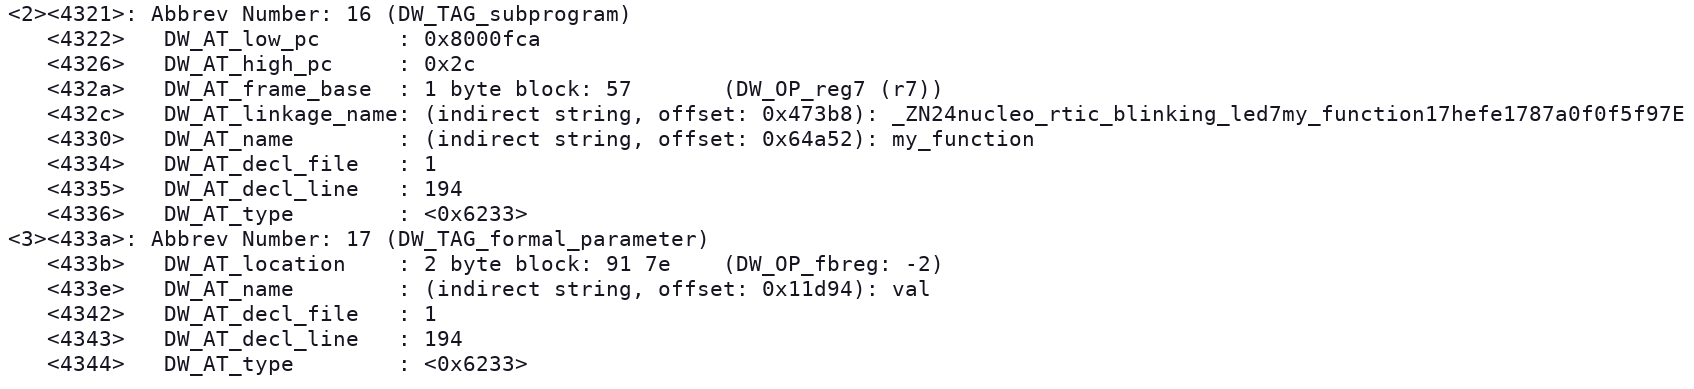
\includegraphics[width=1.0\textwidth]{subprogram-example.png}
	\caption{An example of a subprogram and parameter \gls{DWARF} \gls{die}. This example is the output of the program \emph{objdump} run on a \gls{DWARF} file.}
	\label{fig:subprogramexample}
\end{figure}


\subsubsubsection{Parsing the Raw Value}
Now the fist problem with parsing the raw value of the argument into the correct type is knowing what type the argument has.
Luckily \gls{DWARF} has a attribute for that called \emph{DW\_AT\_type} which value is a offset into the \gls{DWARF} section called \emph{.debug\_types}.
The \emph{val} argument \gls{die} has this attribute and as can be seen in figure \ref{fig:subprogramexample} it has the value $0x6233$ which points to the type \gls{die} seen in figure \ref{fig:basetypeexample}.
Note that the type \gls{die} in the figure has the offset $6233$ which is the same offset that the \emph{val} \gls{die} has in its type attribute.
The type \gls{die} has the tag \emph{DW\_TAG\_base\_type} which means that it a type that is built into the languages and is not defined in terms of other data types(see \cite{dwarf} page 75).
The \gls{die} also have three attributes the first one is the name attributes which in this case says that the base types name is \emph{i16}, see figure \ref{fig:basetypeexample}.
Then there is the attribute \emph{DW\_AT\_encoding} describes how the raw bytes should be interpreted and in this case it has the value $5$ that stands for signed.
Thus from the encoding attribute it is known that the type of \emph{val} is a signed integer, but the size of the integer is still unknown.
The last attribute in the \gls{die} is \emph{DW\_AT\_byte\_size} and it has the value $2$ which means that the size of the signed integer is $2$ bytes.
Now the location, size and type of \emph{val} is known and thus the value can be evaluated.


\begin{figure}[h]
	\centering
	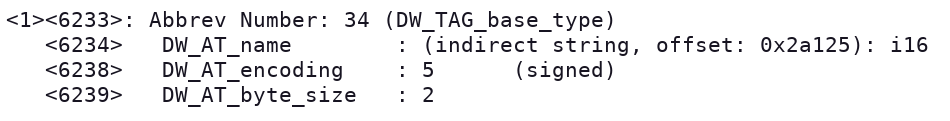
\includegraphics[width=1.0\textwidth]{basetype-example.png}
	\caption{An example of a base type \gls{DWARF} \gls{die}. This example is the output of the program \emph{objdump} run on a \gls{DWARF} file.}
	\label{fig:basetypeexample}
\end{figure}

